\documentclass{beamer}
\mode<presentation> {
\usetheme{Malmoe}
\usecolortheme{whale}
\setbeamertemplate{footline}[page number] 
}
\usepackage{comment}
\usepackage[backend=biber,
style=alphabetic,
citestyle=authoryear
]{biblatex} %Imports biblatex package
\addbibresource{bib.bib} %Import the bibliography file

\title{Estimates in relative survival setting from a counting process point of view}
\author{Yuliya Leontyeva}
\institute{Karolinska Institute, MEB}
\date{{\today}}

\titlegraphic{
\includegraphics[height=1.5cm]{logo.png}\hspace*{-9cm}}





\begin{document}
\maketitle

\begin{frame}
\frametitle{Overview} % Table of contents slide, comment this block out to remove it
\tableofcontents % Throughout your presentation, if you choose to use \section{} and \subsection{} commands, these will automatically be printed on this slide as an overview of your presentation
\end{frame}


\section{Introduction}

\begin{frame}{Introduction}
\small
\begin{itemize}
    \item $N(t)$ is the counting process, the number of events in the observation period $[0; t)$, $t < \infty$ in the cohort:
    $N(t) = \sum_1^n N_i(t)$ the aggregated process
    \item $Y(t)$ is the counting processes of the number at risk corresponding to $N(t)$, where $Y_{i}(t) = I(T_i \geq t)$ is at risk indicator for an individual $i$ in the cohort just before time $t$ 
    \item Under independent censoring the intensity process for an individual $i$  $$\lambda_i(t) = \alpha_i(t) Y_{i}(t)$$
     %Independent censoring is important to have equation (1.20) on page 30 
 \end{itemize}
\end{frame}
 
 \begin{frame}{Introduction. Cont}
 \begin{itemize}
    \item Consider a model with hazard rate:
    \begin{equation}
    \label{eq0}
       \alpha_i(t) = \gamma(t) + \mu_i(t),
    \end{equation} where:
 %The interpretation of the model can be given in a competing risk framework: Each individual is exposed to: a standard risk depending on age, sex, and calendar time and additional risk due to the fact that all individuals suffer from some disease    


     
     $\gamma(t)$ is the excess mortality, assumed to be common to all individuals%, i.e. all individuals are homogeneous
     
     
     $\mu_i(t)$ is mortality rate for a person in the general population corresponding to an individual $i$. This correspondence is usually done due to age, sex and calendar year but there might be other factors too, for example, social status.
     \newline
     Here we denote $\mu_i(t) = \mu_i(a_i + t)$ mortality rate in the general population corresponding to the individual $i$ who were diagnosed at $a_i$ age
     \newline
     Population mortality rate is assumed to be known. 
 \end{itemize}
 \end{frame}
 
 \begin{comment}
 \begin{frame}{Example}
\begin{figure}[hp!]
\centering
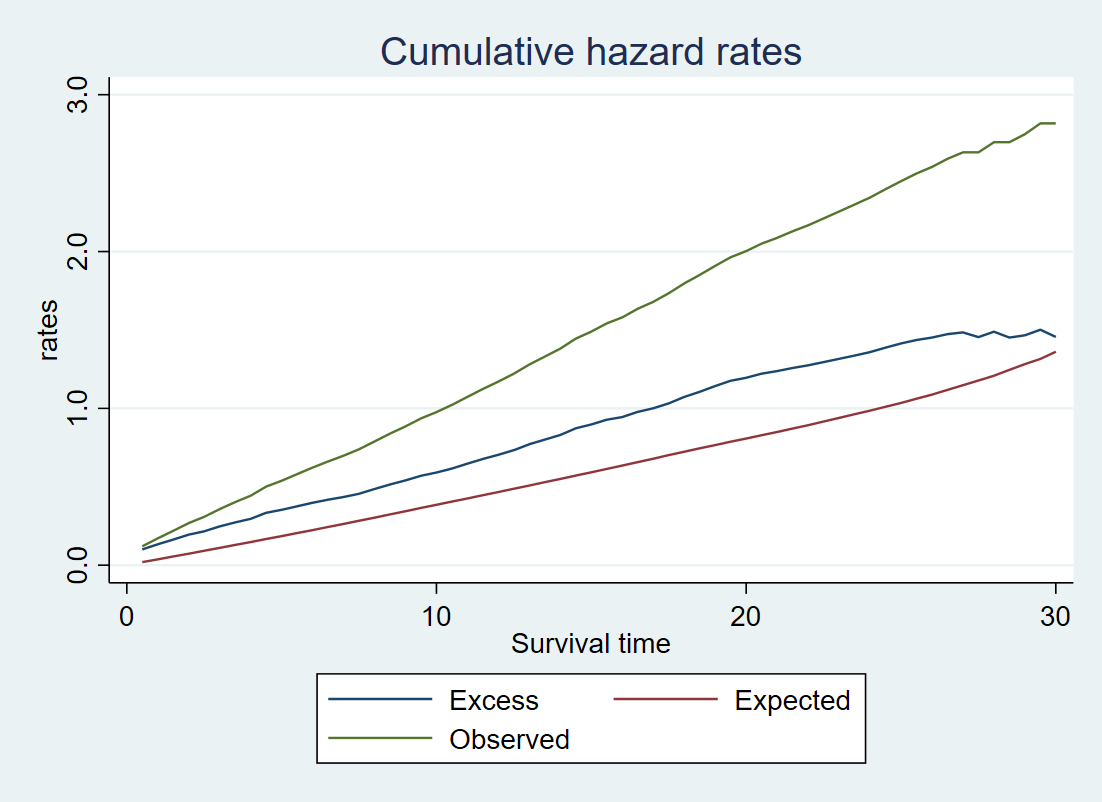
\includegraphics[width=10cm,height = 7cm]{cum_haz.png}
  \label{fig1}
\end{figure}  
% All three curves look roughly linear within about 16 years, indicating that a model with constant excess hazard seems reasonable
\end{frame}
\end{comment}



 \begin{frame}
Then the intensity process for $N(t)$:
\newline

 $\lambda(t) = \sum_i^n \lambda_i(t) = \sum_i^n (\gamma(t) + \mu_i(t)) Y_i(t) \\
 
 = \gamma(t)\sum_i^n Y_i(t) + \sum_i^n \mu_i(t) Y_i(t) = Y(t) (\gamma(t) + \frac{\sum_i^n \mu_i(t) Y_i(t)}{Y(t)} \\
    
    
     = Y(t) (\gamma(t) + \bar\mu(t))$
 
  \end{frame}
  
  \begin{frame}{Introduction. Cont}
  \begin{itemize}
      \item $\lambda(t) = Y(t) (\gamma(t) + \bar\mu(t)),$ 
      where 
     \begin{equation}
     \label{eq1}
     \bar\mu(t) = \sum_i^n \mu_i(a_i+t) \frac{Y_i(t)}{Y(t)}
     \end{equation}
   \newline
     is the average population mortality among the individuals at risk just before time t.
    % This is an average because we divide population mortality $\mu_i(t)Y_i(t)$ with Y(t)-total number at risk at time t.$
   \end{itemize}
\end{frame}

\begin{comment}
\begin{frame}{Introduction. Cont}
    If we assume parametric distribution for the hazard rate with a parameter $\theta$ (which can be, of course, a vector of parameters), then the likelihood can be written in terms of product integral:
    \begin{equation}
        L(\theta) =  \pi (\prod_{i=1}^n (\lambda_i(t)^{\Delta N_i(t)}) x (1-\lambda(t)dt)^{1-\Delta N(t)}) \\\
    = \pi (\prod_{i=1}^n((\gamma(\theta,t) + \mu_i(t))Y_i(t))^{\Delta N_i(t)}) x (1 - \lambda(t)dt)^{1-\Delta N(t)})
    \end{equation}
    \newline
    \newline
    \cite{andersen}, p 99, equation 2.7.2''
    
\end{frame}
\end{comment}



\section{The estimate of cumulative excess mortality and its properties}
  \begin{frame}{The cumulative excess mortality}
 \begin{itemize} 
   \item $dN(t) = \lambda(t)dt + dM(t) = Y(t) (\gamma(t) + \bar\mu(t)) dt + dM(t)$ is an incremenent of the counting process
   \newline
   \item $\frac{J(t) dN(t)}{Y(t)} = J(t)(\gamma(t) + \bar\mu(t)) dt + \frac{J(t)dM(t)}{Y(t)}$
   \end{itemize}
\end{frame} 
   
   \begin{frame}{The cumulative excess mortality. Cont}
   \begin{itemize} 
   \item $\int_0^t \frac{J(s)}{Y(s)}dN(s) = \int_0^t J(s)\gamma(s) ds + \int_0^t J(s)\bar\mu(s)ds + \int_0^t \frac{J(s)dM(s)}{Y(s)}$
   \newline
   \item $\hat A(t) = \Gamma^*(t) + \int_0^t J(s)\bar\mu(s)ds + \int_0^t \frac{J(s)dM(s)}{Y(s)}$ 
   %Nelson_Aalen estimator
    \item $\hat\Gamma(t) = \hat A(t) - \int_0^t J(s) \bar\mu(s) ds,$
   \newline
   which is unbiased estimator of $\Gamma^*$.
   %because $\int_0^t \frac{dM(s)}{Y(s)}$ is a stochastic integral with respect to martingale, i.e. it is zero-mean martingale.
  \newline
  \newline
   Thus, the estimator for the cumulative excess mortality is the difference between the Nelson-Aalen estimator for the group under study and the cumulative average population mortality.
   \end{itemize}
\end{frame}

\begin{frame}{Variation process}
\begin{itemize}
  \item We use the optional variation process as an estimator of the variance of the cumulative excess hazard $$[\int HdM](t) = \int_0^t H^2(s) dN(s) $$
 \begin{equation}
 \label{eq3}
      [\hat\Gamma - \Gamma^*](t) = \int_0^t \frac{J(s)}{Y_1(s)^2} dN_1(s),
 \end{equation}
 \newline 
 This is unbiased estimator, because
 $$Var(\hat\Gamma(t) - \Gamma^*(t)) = Var(\hat\Gamma(t)) = E[\hat\Gamma - \Gamma^*](t) = E(\int_0^t \frac{J(s)}{Y_1(s)^2} dN_1(s)) $$
 \newline
 $ Var(\hat\Gamma(t)) = Var( \hat A(t) - \int_0^t J(s) \bar\mu(s) ds) = Var(\hat A(t)) = \int_0^t \frac{J(s)}{Y_1(s)^2} dN_1(s) ,$
 
 %because mortality rates in the general population are assumed to be known
     
\end{itemize}
\end{frame}

\section{Asymptotic properties}
\subsection{Uniform consistency}
\begin{frame}{Uniform consistency}
\begin{itemize}
\item Consider a sequence of counting processes $N^{(n)} = (N_1^{(n)},N_2^{(n)}, ..., N_k^{(n)})$
\item We should show that $sup|\hat\Gamma^{(n)}(t) - \Gamma^*(t)| \rightarrow 0$  
\item We use the Lenglart's inequality that for any $\epsilon$,$\tau > 0$:
$$P(sup(\int_0^t H(s)dM(s)ds)^2  \geq \epsilon) \leq \frac{\tau}{\epsilon} + P(\int_0^T H^2(s)d<M>(s) \geq \tau) $$
\newline
where $T$ is a stopping time.
\end{itemize}
 \end{frame}


\begin{frame}{Uniform consistency.Cont}
\begin{itemize}
\item Recall, $$\hat\Gamma(t) - \Gamma^*(t) = \int_0^t \frac{dM(s)}{Y(s)} = \int_0^t H(s) dM(s)$$
\item $\int_0^t H(s) dM(s)$ is a zero-mean martingale
\item Using that $E|M| =\sqrt{E(M^2)}$, hence $E(M^2) = (E|M|)^2$  
\item $sup|\hat\Gamma^{(n)}(t) - \Gamma^*(t)| = sup(M^2) = sup (\int_0^t H(s) dM(s))^2$
%therefore $(\int_0^t H(s) dM_1(s))^2$ is a submartingale (Jensen's inequality).
% \int_0^t H(s) dM(s) = M, (\int_0^t H(s) dM(s))^2 = M^2
%$E(M^2(t)|F_s) \geq (E(M(t)|F_s))^2 = M^2(s)$
%\item By Doob-Meyer decomposition, there is a unique compensator (predictable process) for $M^2(t)$: $<M>(t)$
\end{itemize}
 \end{frame}


\begin{frame}{Uniform consistency. Cont}
If we look at the right side of the Lenglart's inequality: 
\begin{itemize}
  \item $<M>(t) = < \int_0^t H(s) dM(s) > \leq \int_0^T H^2(s) d<M>(s) \\\
= \int_0^T \frac{1}{Y(s)^2}\lambda(s)ds = \int_0^T \frac{\alpha(s) Y(s)ds}{Y(s)^2} \leq \int_0^T \frac{\alpha(s)}{Y(T)} = \frac{A(T)}{Y(T)},$ \\\
\newline
where $T$ is stopping time.
\newline
When $n \rightarrow \infty,$ then $Y(T) \rightarrow \infty$ and  $<M>(t) \rightarrow 0$.
% equation (2.29) 
\newline
\newline
Thus, $P(\int_0^T H^2(s)d<M>(s) \geq \tau) \rightarrow 0$


\end{itemize}
\end{frame}

\begin{frame}{Uniform consistency.Cont}
Finally, using that $M^2 - < M>$ is a zero mean martingale,
\newline
\newline
$P(sup(\int_0^t H(s)dM(s)ds)^2  \geq \epsilon) \leq \frac{\tau}{\epsilon} + P(\int_0^T H^2(s)d<M>(s) \geq \tau) \\\ 
= P(sup(\int_0^t H(s)dM(s)ds)^2  \geq \epsilon) - P(\int_0^T H^2(s)d<M>(s) \geq \tau) \leq \frac{\tau}{\epsilon},$ \\\

where,
\newline
$P(sup(\int_0^t H(s)dM(s)ds)^2  \geq \epsilon) - P(\int_0^T H^2(s)d<M>(s) \geq \tau) \rightarrow 0$ 
and 
\newline
$P(\int_0^T H^2(s)d<M>(s) \rightarrow 0 $ 

If we take $\tau$ and $\epsilon$ small,
$$sup|\hat\Gamma(t) - \Gamma^*(t)| \rightarrow 0,$$ when $n \rightarrow \infty$, i.e. we have uniform consistency  
\end{frame}


\subsection{Asymptotic distribution}
\begin{frame}{Asymptotic distribution}
$\hat\Gamma(t) - \Gamma^*(t) = \int_0^t \frac{J(s) dM(s)}{Y(s)}$ is a mean-zero martingale
\newline
\newline
To apply Martingale central limit theorem, check conditions:
\begin{itemize}
    \item $H(s)^2 \lambda(s) \rightarrow v(s),$ where $v(s)$ a deterministic function
    \item H(s) converges in probability to 0.
\end{itemize}
\end{frame}
   
\begin{frame}{Asymptotic distribution. Cont}
Can we scale $\hat\Gamma(t) - \Gamma^*(t)$ in a way to apply Martingale central limit theorem? If we consider:
$\sqrt{n}(\hat\Gamma(t) - \Gamma^*(t))$ is a Wiener process  
\newline
Analogically to Nelson-Aalen estimator in lectures, we get:
\newline
\begin{itemize}
    \item $H(s)^2 \lambda(s) =(\sqrt{n})^2 \frac{J(s)Y(s)\alpha(s)}{Y^2(s)} = n\frac{J(s)Y(s)(\gamma(s) + \bar\mu(s)}{Y^2(s)} \\\
    = \frac{J(s)(\gamma(s)+\bar\mu(s))}{Y(s)/n}$
    \newline
    \newline
    Assume that $\frac{\gamma(s) + \bar\mu(s)}{Y(s)/n} \rightarrow \frac{\gamma(s) + \bar\mu(s)}{y(s)} ,$ when $n \rightarrow \infty$, i.e. $v(s) = \frac{\gamma(s) + \bar\mu(s)}{y(s)}$ and $y(s) > 0$
    
    
    \item $\sqrt{n}\frac{J(s)}{Y(s)} = \frac{J(s)}{\sqrt{n}} \frac{1}{Y(t) / n} \rightarrow 0,$ when $n \rightarrow \infty$
    
\end{itemize}
\end{frame}

\begin{frame}{Asymptotic distribution. Cont}
Thus, according to martingale central limit theorem, $\sqrt{n}(\hat\Gamma(t) - \Gamma^*(t))$ converges to Gaussian zero-mean distribution with variance function $V(t) = \int_0^t v(s) ds = \int_0^t \frac{\gamma(s) + \bar\mu(s)}{Y(s)}ds$ and estimated by (\ref{eq3}).
%which is unbiased estimator
\newline
\newline
Analogically to the lectures, asymptotically there is no difference between $\Gamma(t)$ and $\Gamma^*(t)$ because as $\frac{Y(t)}{n} \rightarrow y(t),$ when $n \rightarrow \infty$ and $y(t) > 0$, then $J(t) \rightarrow 1$ 
%J(t) is an indicator and if asymptotically y(t) strictly bigger than zero then indicator will be always 1, it is 0 only when y(t) = 0
\newline   
\newline
I.e. there is only a small probability that there is no one at risk at times $s \leq t$.
\end{frame}

\subsection{Some interesting findings}
\begin{frame}{Some interesting findings}
\begin{itemize}
\item $E(Y(t))$ is the expected number still at risk just before time $t$. 
    \item The bias of $\hat A(t)$ is less than 0.25\% as long as $E(Y(t)) \geq 3$
    \item The variance estimator (\ref{eq3}) overestimates the true variance but the bias does not exceed 5\%  as long as $E(Y(t)) \geq 3$ 
    \item \cite{andersen}, p.182
\end{itemize} 
   
\end{frame}

\section{The estimate of the relative survival}
\begin{frame}{Corresponding survival function}
\begin{itemize}
\item Recall that
%the relationship between between S and cumulative hazard can be expressed in terms of product integral (Appendix A.1)
%Product integral is not any continuous integration, it is when $n \rightarrow \infty$, the width of the interval goes to 0
$S(t) = \Pi_{u \leq t}(1-dA(u))$.
\newline
For a continuous function $dA(u) = \alpha(u)du$ and using approximation $exp(\alpha(u)du) \approx 1+ (-\alpha(u)du)$ we obtain that 
$$S(t) = exp(-A(t))$$
\item Excess hazard is decomposed as: $\hat\Gamma(t) = \hat A(t) - A_p(t),$ then 
\newline
$\hat RS = exp(-\hat A(t) - (-A_p(t))) = \frac{exp(-\hat A(t))}{exp(-A_p(t))} = \frac{\hat S(t)}{S_e(t)} =\frac{exp(-\hat A(t))}{exp(\int_0^t \bar \mu (s) ds)} $ 
%Relative survival cannot be interpreted as survival probability because, excess hazard can be negative and increasing and RS can be bigger than 1 if the group has the mortality lower than in the general population
% S(t) is Kaplan-Meier for the group under study
% Expected survival function, i.e. the survival function one would have if the mortality in the group had been the same as in the general population (conditional on the observed number at risk)
% Other definitions of expected survival curves are also available
% In RS estimator both cumulative hazards are considered to be continuous
% a continuous-time generalization of the expected survival curve is obtained as a by-product.
\end{itemize}
\end{frame}

\begin{frame}{Corresponding survival function}
Recall that the mortality rate in the general population is assumed to be known, the statistical properties of $RS$ estimator can be studied in the same way as for $KM$ estimator, i.e.
\begin{itemize}
    \item $RS$ is almost unbiased when there is only a small probability that there is no one at risk at times $u \leq t$
    \item $Var(\hat RS) = \frac{Var(\hat S(t))}{S_e(t)^2}  = \frac{\hat S(t)^2 Var(\hat A(t))}{S_e(t)^2} = \hat RS(t)^2  Var(\hat A(t))$
\end{itemize}

\end{frame}

\section{Additive non parametric excess hazards models}
\begin{frame}{Additive excess hazards model}
Using (\ref{eq0}) individual hazard rate can be written:
$$\alpha_i(t|x_i) = \beta_0(t) + \beta_1(t)x_{i_1} + ... + \beta_p(t)x_{i_p} + \mu_i(a_i + t) = X(t)\beta(t) + \mu_i(a_i + t) $$
$\beta_0(t)$ is the baseline hazard rate, 
%corresponding to the hazard rate of an individual with all covariates equal to 0.
$\beta_j(t)$ is the increase in the hazard at time $t$
%corresponding to unit's increase
and $\beta_j(t)$ are arbitrary regression functions.
We want to estimate a cumulative regression function for each $\beta_j(t)$, $$B_j(t) = \int_0^t \beta_j(s)ds,$$ where $j=0,...,p$
\end{frame}

\begin{frame}
We define a modified counting process:
$\widetilde{N(t)} = N(t) - \Lambda^*,$ where
$\Lambda^* = \int_0^t \lambda_i^*(s)ds$ and $\lambda_i^*$ is intensity in the general population.
$$\lambda(t) = \textbf{Y(t)} \alpha(t),$$
where $\textbf{Y(t)}$ is $n x (p+1)$ matrix with row $i$ equal to $Y_i(t) = I(T \geq t)(1,x_{i1},...,x_{ip})$ 
\newline
$$d\widetilde{N(t)} = dN(t) - \lambda^*(t)dt = \lambda(t)dt + dM(t)- \lambda^*(t)dt \\\
= (\lambda^*(t) + Y(t)\beta(t))dt - \lambda(t)^*dt + dM(t) = Y(t)\beta(t)dt + dM(t)$$
\newline
\newline
%$[\Lambda^*(s) = \int_0^t \lambda^*(s) ds, d\Lambda^*(t) = \lambda^*(t)dt]$
\end{frame}

\begin{frame}{Additive excess hazards model. Cont}
$$d\widetilde{N(t)} = Y(t)\beta(t)dt + dM(t)$$
We obtain:
\begin{equation}
\label{eq5}
    \hat B^*(t) = \int_0^t Y(t)^{-}d\widetilde{N(t)}
\end{equation}
where $Y^{-}$ is a predictable generalized inverse, which using least squares principle applied to the linear equations equals:
$$Y^{-}(t) = (Y(t)^TY(t))^{-1}Y(t)^T $$
\end{frame}

\begin{frame}
Equation (\ref{eq5}) can be rewritten:
$$\hat B^*(t) = \int_0^t Y^-(s)dN(s) - \int_0^t Y(t)^{-}\lambda^*(s)ds
= \hat B(t) - \int_0^t Y(t)^{-}\lambda^*(s)ds,$$
 is the difference of Aalen estimator and a predictable term depending on the background mortality rate and the observed covariates in the data. 
   \end{frame}


%\section{Unknown population mortality}
\begin{frame}{The estimate of cumulative excess mortality with unknown population mortality. Extra}
Assume now that $\mu_i(t^*)$ is unknown. Here $t^*$ is the time from the birth of an individual in the general population
\newline
If we define $N_{2_i}$ is a counting process of an individual in a small interval $[t^*; t^*+\Delta t^*)$, then $N_{2_j_\bullet}$ is an aggregated counting process, the number of deaths among individuals at age $a_j$ in the general population.
\newline
%These processes are independent of the excess mortality in the given cohort. 
\newline
Its intensity can be written:
$$\lambda^*_j(t^*)=Y_{2_j_\bullet}(t^*)\mu_j(t^*)$$

i.e. we assume that within age group population mortality rates are the same
\end{frame}


\begin{frame}{The estimate of cumulative excess mortality with unknown population mortality. Extra}
We can obtain a point estimator for mortality rates within one age group:
\begin{equation}
\label{eq2}
    \hat \mu_j(t^*) = \frac{N_2_j_{\bullet}}{Y_2_j_{\bullet}},
\end{equation}
 \newline
 %where $N_2_{\bullet}$ is the total number of all event in the general population for individuals of age, sex and calendar year, corresponding to the individual $i$ in the cohort and $Y_2_{\bullet}$ is the total person-time in each group.
 \newline
We can then plug-in the estimates (\ref{eq2}) to the equation (\ref{eq1}) 
\newline
We also get an unbiased estimator of $\Gamma^*$
\end{frame}

\begin{frame}{Variation process. Extra}
If we assume again that the population mortality rates are unknown. Then: $M = M_1 + M_2$ and 
$$[\hat\Gamma(t) - \Gamma^*(t)] = [M_1 + M_2]$$
Then:
$$<M_1 + M_2> = <M_1> + <M_2> + 2<M_1,M_2>, $$
where $M_1$ and $M_2$ are martingales of the corresponding counting processes: $N_1$, the number of events due to "cancer" and $N_2$, the number of events due to other reasons.  
\newline
Note, that $N_1$ and $N_2$ do not jump simultaneously (assumption which is proved to be reasonable). But then $<M_1,M_2>$ = 0. 
\end{frame}

\begin{frame}
    $Var(\hat \Gamma(t)) = Var( \hat A(t)) + Var(\int_0^t J(s) \bar\mu(s) ds)) + 2Cov(\hat A(t),\int_0^t J(s) \bar\mu(s) ds)) \\\

= \int_0^t \frac{J(s)}{Y(s)^2} dN(s) + Var(\int_0^t \sum_{i=1}^n \frac{N_2_i_{\bullet}}{Y_2_i{\bullet}}\frac{J(s)Y_1_i(s)}{Y_1(s)}) + 2 Cov(...) \\\
= \int_0^t \frac{J(s)}{Y(s)^2} dN(s) + \int_0^t \sum_{i=1}^n \frac{J(s)Y_1_i(s)}{Y_1^2(s)}\frac{N_2_i{\bullet}}{Y_2_i{\bullet}} + 2Cov(...) $
\end{frame}




\begin{frame}{Variation process. Extra}
If we assume that both $\mu$ and $\gamma$ are constant. 
\begin{align*}
\hat\gamma &= \frac{N_{1\bullet}}{Y_{1\bullet}} - \frac{N_{2\bullet\bullet}}{Y_{2\bullet\bullet}} \\
  \hat\mu &= \frac{N_{2\bullet\bullet}}{Y_{2\bullet\bullet}} \\
  Var(\hat \gamma) = \frac{N_{1\bullet}}{Y_{1\bullet}^2} + \frac{N_{2\bullet\bullet}}{Y_{2\bullet\bullet}^2}
\end{align*}
I.e. the variance of excess hazard in this case is the variance of the observed process and the variance of the process in the general population.
\end{frame}



\begin{frame}{Bibliography}
\printbibliography %Prints bibliography
\end{frame}

\end{document}

 The article which I can read only online
https://www.jstor.org/stable/4616409?read-now=1&seq=1#page_scan_tab_contents